\subsection{Results}\label{sec:tauResults}

\subsubsection{2010 signal region}
\begin{figure}[hbtp]
  \subfigure[]{\label{fig:tauMET2010}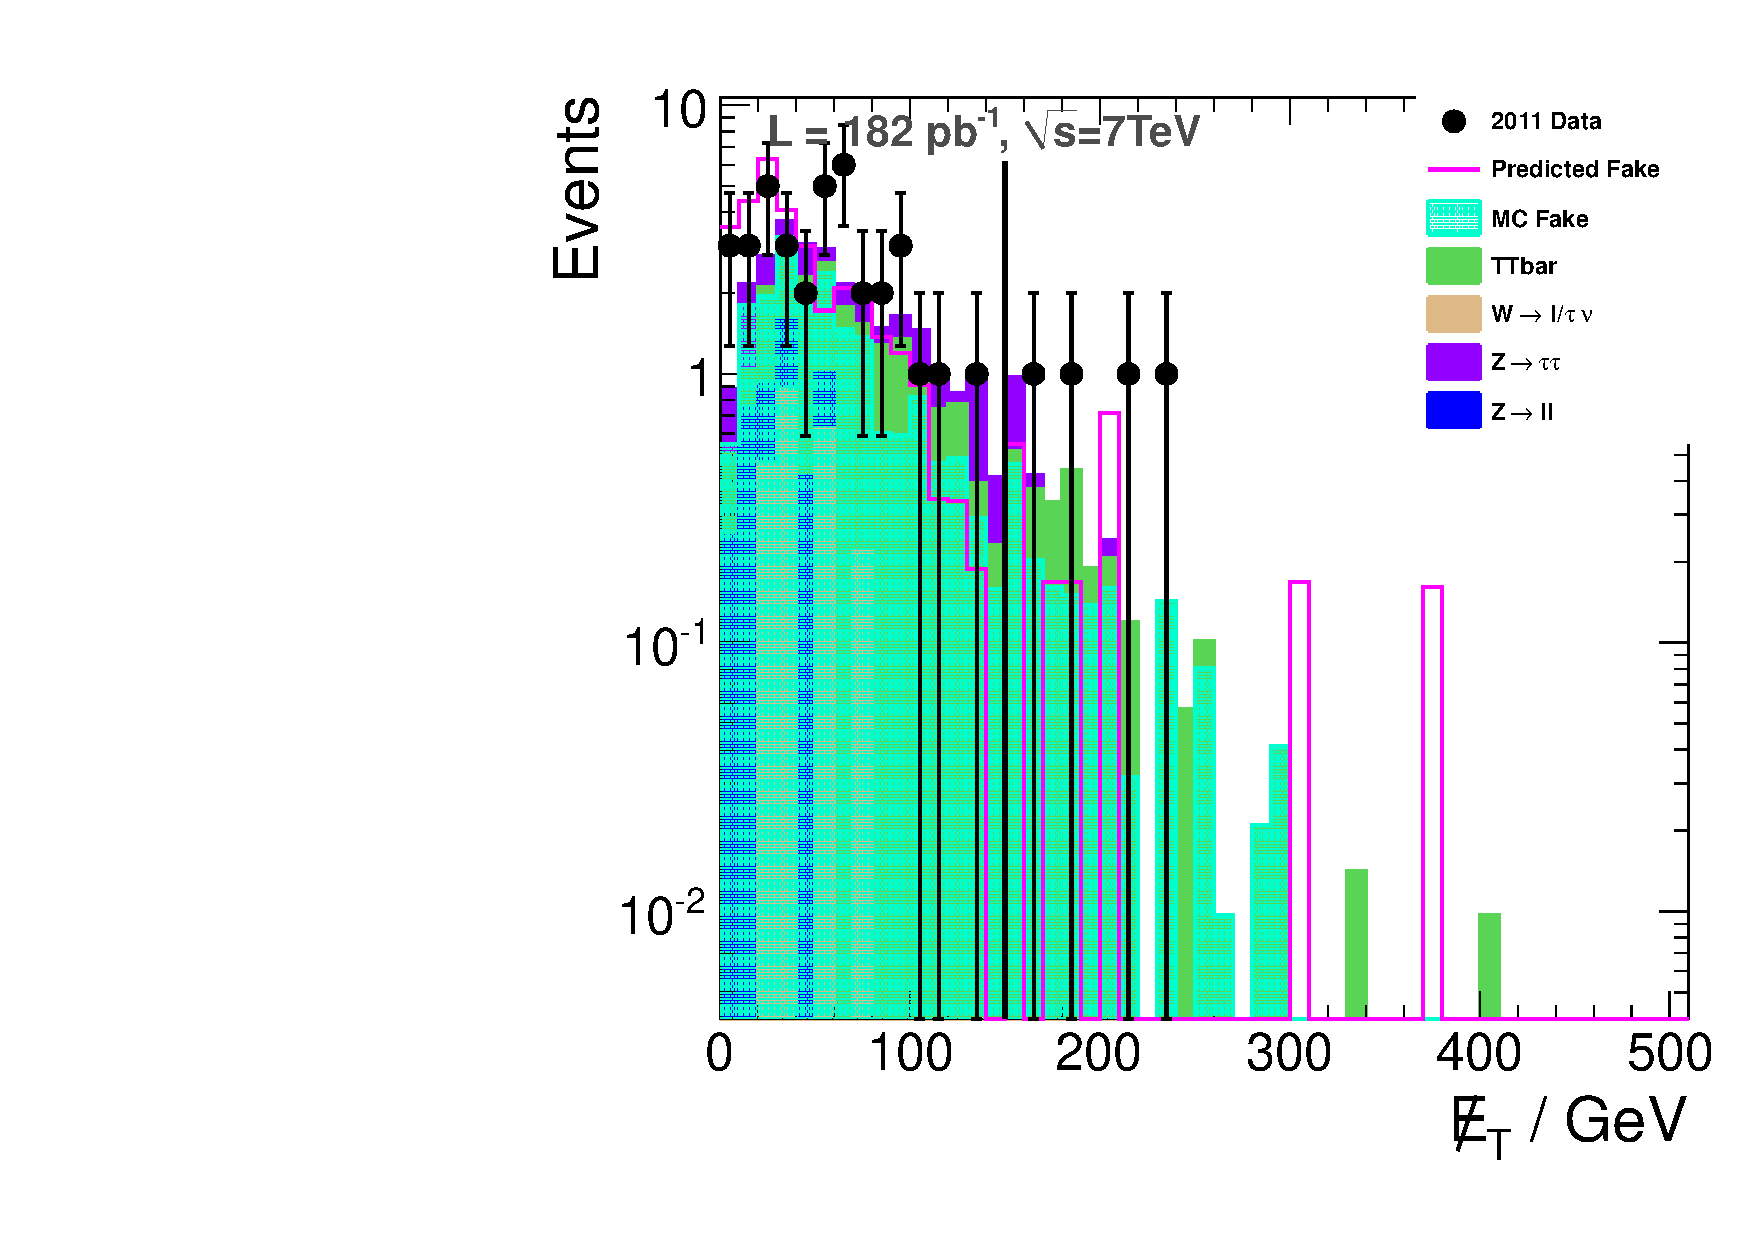
\includegraphics[width=0.79\textwidth]{plots/HighPt-2010Selection-anyTau-met.pdf}}\hfill
  \caption{\MET distribution for all events passing e$\tau$ or $\mu\tau$ selection and satisfy $\HT> 350$~GeV. For the final \MET selection (150)~GeV the selection is dominated by $t\bar{t}$.}
\end{figure}

The \MET distribution after application of the \HT
cut is shown in Fig~\ref{fig:tauMET2010} and
the yield split by flavour for a cut at 150~GeV is listed in Tab.~\ref{tab:tau2010}.

\begin{table}[htb]
\begin{center}
\caption{\label{tab:tau2010}\protect Summary of number of events expected from Monte Carlo simulations in 
the signal region of $H_T> 350$~GeV and $\MET> 150$~GeV.}

\begin{tabular}{l|c c |c}
Sample & e$\tau$ & $\mu\tau$ & total\\
\hline
Z $\rightarrow$ ll & $< 0.1$ & $< 0.1$ & $< 0.1$\\
Z $\rightarrow$ $\tau$$\tau$ & $< 0.1$ & $0.1$ & $0.1$\\
TTbar & $1.2$ & $1.3$ & $2.5$\\
W $\rightarrow$ l/$\tau$ $\nu$ & $0.2$ & $< 0.1$ & $0.2$\\
$\sum SM$ & 1.4 & 1.4 & 2.8\\
\hline
2011 Data & $2.0$ & $2.0$ & $4.0$\\
\hline
\hline
Predicted Fake & $0.7$ & $1.2$ & $1.9$\\
Prompt TTbar   & $0.6$ & $0.5$ & $1.0$\\
\hline
MC Fake & 0.9 & 0.8 & 1.6 \\
\end{tabular}
\end{center}
\end{table}

\subsubsection{High \HT signal region}
\begin{figure}[hbtp]
  \subfigure[]{\label{fig:tauMETHighHT}\includegraphics[width=0.79\textwidth]{plots/HighPt-highHt-anyLTau-met.pdf}}\hfill
  \caption{\MET distribution for all events passing e$\tau$ or $\mu\tau$ selection and satisfy $\HT> 600$~GeV. For the final \MET selection (100)~GeV the selection is dominated by $t\bar{t}$.}
\end{figure}

The \MET distribution after application of the \HT
cut is shown in Fig~\ref{fig:tauMETHighHT} and
the yield split by flavour for a cut at 100~GeV is listed in Tab.~\ref{tab:tauHighHT}.

\begin{table}[htb]
\begin{center}
\caption{\label{tab:tauHighHT}\protect Summary of number of events expected from Monte Carlo simulations in 
the signal region of $H_T> 600$~GeV and $\MET> 100$~GeV.}
\begin{tabular}{l|c c |c}
Sample & e$\tau$ & $\mu\tau$ & total\\
\hline
Z $\rightarrow$ ll & $< 0.1$ & $< 0.1$ & $< 0.1$\\
Z $\rightarrow$ $\tau$$\tau$ & $0.1$ & $< 0.1$ & $0.1$\\
TTbar & $0.8$ & $0.4$ & $1.2$\\
W $\rightarrow$ l/$\tau$ $\nu$ & $0.2$ & $< 0.1$ & $0.2$\\
$\sum SM$ & 1.1 & 1.4 & 1.5\\
\hline
2011 Data & $0$ & $1$ & $1$\\
\hline
\hline
Predicted Fake & $0.2$ & $0.3$ & $0.5$\\
Prompt TTbar  & $0.5$ & $0.1$ & $0.6$\\
\hline
MC Fake & 0.3 & 0.1 & 0.4\\
\end{tabular}
\end{center}
\end{table}

\subsubsection{High \MET signal region}
\begin{figure}[hbtp]
  \subfigure[]{\label{fig:tauMETHighMET}\includegraphics[width=0.79\textwidth]{plots/HighPt-highHt-anyLTau-met.pdf}}\hfill
  \caption{\MET distribution for all events passing e$\tau$ or $\mu\tau$ selection and satisfy $\HT> 250$~GeV. For the final \MET selection (250)~GeV the selection is dominated by $t\bar{t}$.}
\end{figure}

The \MET distribution after application of the \HT
cut is shown in Fig~\ref{fig:tauMETHighMET} and
the yield split by flavour for a cut at 250~GeV is listed in Tab.~\ref{tab:tauHighMET}.

\begin{table}[htb]
\begin{center}
\caption{\label{tab:tauHighMET}\protect Summary of number of events expected from Monte Carlo simulations in 
the signal region of $H_T> 250$~GeV and $\MET> 250$~GeV.}
\begin{tabular}{l|c c |c}
Sample & e$\tau$ & $\mu\tau$ & total\\
\hline
Z $\rightarrow$ ll & $< 0.1$ & $< 0.1$ & $< 0.1$\\
Z $\rightarrow$ $\tau$$\tau$ & $0.1$ & $< 0.1$ & $0.1$\\
TTbar & $0.1$ & $0.1$ & $0.2$\\
W $\rightarrow$ l/$\tau$ $\nu$ & $0.2$ & $< 0.1$ & $0.2$\\
$\sum SM$ & 0.4 & 0.1 & 0.5\\
\hline
2011 Data & $0.0$ & $0.0$ & $0.0$\\
\hline
\hline
Predicted Fake & $< 0.1$ & $0.3$ & $0.3$\\
Prompt TTbar & $< 0.1$ & $0.1$ & $0.2$\\
\hline
MC Fake & 0.2 & 0.1 & 0.3\\
\end{tabular}
\end{center}
\end{table}

